%************************************************
\chapter{Implementation}\label{ch:implementation}
%************************************************
This chapter explains the implementation of the proposed solution in \autoref{ch:design}. The first section of this chapter explains the relevant technologies with several details about the communication. Additionally, several decisions are described in \autoref{sec:exposing_data}. This chapter is finished with a deployed demo application which verifies the effectiveness of the implemented solution (\autoref{sec:demo_app}).

\section{Interface} \label{sec:interface}
As explained in \autoref{sec:architecture}, the proposed solution consists of three different types. This section provides an overview of each type and the communication between them.

\subsection{Root} \label{sec:impl-root}
The root contains the connect API which is used as an access point for other nodes. Its interface contains the following relevant endpoints:

\begin{itemize}
    \item \textbf{/root/add}: accepts POST-requests for adding nodes to keep track of. A node consists of an IP-address, including a port, and a boolean value indicating whether it is a super-node or a normal node.
    \item \textbf{/root/remove}: accepts POST-requests for removing nodes from the list. All properties from the previous endpoint must be equivalent before the node is removed. Additionally, this service pings every node once in a while to ensure that the node can still be accessed. If a node cannot be accessed for $X$ pings in a row (with an interval of $Y$ seconds), the node is removed from the list.
    \item \textbf{/root/distribution}: accepts a GET-request for returning the distribution. The endpoints returns therefore a list of all super-nodes with a list of all the nodes that are scraped by the super-nodes. Note that each super-node is also updated with the new distribution as soon as a new (super-)node is added to the list. 
\end{itemize}

\noindent
The root service is a rather small service as it only has to keep track of the available (super-)nodes and distribute them over the available super-nodes. This service is implemented at \url{https://github.com/dadvisor/root}. The root service also provides a dynamic configuration of the Prometheus service. This is implemented by generating a configuration file with the addresses of the super-nodes. Prometheus is configured by reading his configuration from this file.\\

\noindent
Lastly, the root-type contains the Grafana dashboard. This service uses a custom designed dashboard, which is publicly available at \url{https://grafana.com/dashboards/10286}. Grafana is configured in such a way that it automatically adds the local Prometheus service as a data source and installs the dashboard mentioned above. The dashboard uses not only existing visualization tools like graphs and singlestat-panels, but it also visualizes the cost and waste data in a custom designed panel.\\

\noindent
This panel is implemented in the typescript programming language and can its source code can be found at \url{https://github.com/dadvisor/containers-panel}. It generates 17 different graphs that can all be used to investigate which services (or group of services) are responsible for consuming the most cost or waste. This can also be generated per resource metric as explained in the pricing model (\autoref{sec:pricing}). The graphs for a demo application are presented in \autoref{sec:demo_app}.

\subsection{node} \label{sec:node_imp}
The node is the probe that collects information about the host that serves the cloud application. Therefore, the node must be deployed on every host that belongs to the cloud system. To summarize, its responsibilities are the following:
\begin{enumerate}
    \item Inspect internet packets and analyse these to find out which containers are communicating with each other.
    \item Identify the running containers, including their IP addresses. Collect resource statistics about the running containers.
    \item Expose the collected data in a specific format, such that it can be used by Prometheus.
\end{enumerate}

\noindent
In case of being a supernode, it also needs to known its children for scraping data. Therefore, it needs to communicate with the root to find out this information. Below is a short overview of each of the tasks defined above.

\subsection{Identify internet traffic} \label{sec:identify-traffic}
Internet traffic monitoring needs to be optimized as much as possible, as it is not unusual to send thousands of packets a second per node. Therefore, several optimizations are used, which are described below.\\

\noindent
First of all, the TCPdump command uses several arguments to filter out messages that cannot be resolved. The entire command can be found below.
\begin{verbatim}
tcpdump -c TRAFFIC_K -i any -nn ip and -l -t not port 14100 and
tcp and (((ip[2:2] - ((ip[0]&0xf)<<2)) - ((tcp[12]&0xf0)>>2))
 != 0)
\end{verbatim}
An explanation of the arguments can be found below:
\begin{itemize}
    \item \textbf{-c TRAFFIC\_K}: collect a configurable amount of packets and then stop. The default value is $1000$.
    \item \textbf{-i any}: Any interface \cite{tcpmanpage}.
    \item \textbf{-nn ip}: Don't convert addresses (i.e., host addresses, port numbers, etc.) to names \cite{tcpmanpage}.
    \item \textbf{-l}: Make the output line buffered.
    \item \textbf{-t}: Don't print the timestamp, as this is not used.
    \item \textbf{not port 14100}: this port is filtered, as this is the default port for communicating with the node. This option can be configured, such that is contains more ports.
    \item \textbf{tcp} Only retrieve TCP data.
    \item \textbf{$(\dots~~!= 0)$}: Filter packets with a content length of $0$ \cite{tcpdump-filter}.
\end{itemize}
An example of the output of the TCPdump is provided below. This data is generated using two containers. The first container continuously sends a request, while the second container answers this.
\begin{verbatim}
IP 172.18.0.3.36754 > 172.18.0.2.6000: Flags [P.], seq
1926123634:1926123773, ack 2643836746, win 229, option
[nop,nop,TS val 132941 ecr 132941], length 139

IP 172.18.0.2.6000 > 172.18.0.3.36754: Flags [P.], seq
154:156, ack 139, win 235, options [nop,nop,TS val 132940 
ecr 132937], length 2
\end{verbatim}
From this data, the following information can be extracted:
\begin{itemize}
    \item The first line of data contains the request message, while the second line of data contains the response message.    
    \item The container opens port 36754 for sending the request.
    \item The web-service reads and answers on port 6000.
    \item Now it can be concluded that port 6000 belongs to the web-service, with IP 172.18.0.2. Therefore, the request container must use IP 172.18.0.3.
\end{itemize}
It is important to understand the IP addresses of the TCP packet, as this reveals the direction of the packet. There are three cases possible:
\begin{itemize}
    \item Both the source and destination are on the same host. Now, both addresses need to be resolved into a container ID. This is already shown in the example above.
    \item The source is a remote location and the destination is on the host. In this case, the destination needs to be resolved into a container ID.
    \item The source is located on the host and the destination is remote. In this case, the source needs to be resolved into a container ID.
\end{itemize}

\noindent
In case of a remote address, it either originates from another node in the system, or originates from an external address. In the former, the system can communicate with the node to verify the container ID. In the latter, it is not necessary to investigate further. In order to find out whether the data is internal, a list of internal nodes must be known.\\

\noindent
The decision whether data is internal (i.e. between two containers on the same host) or external is not sufficient. In the former case, the data needs to be connected to a container ID. In order to do so, each node must keep track of a list of containers and ports. Given the following example, the list contains the following item: port 6000 belongs to IP 172.18.0.2.
\begin{verbatim}
IP 10.164.0.8.53512 > 172.18.0.2.6000 ... length 82
\end{verbatim}

\noindent
This example above also shows that if the IP address is remote (and from another node), then the nodes can communicate with each other to find out which container ID belongs to port 53512.
To summarize, each node needs to keep track of two mappings. First of all, a mapping from port to IP address. Using the IP address, the node can find out which container belongs this. This is the second mapping.

\subsection{Identify containers}
In order to find out the containers that are currently running, the following command is used:
\begin{verbatim}
curl -s --unix-socket 
/var/run/docker.sock http://localhost/containers/json
\end{verbatim}

\noindent
This command communicates with the Docker API and returns a list of containers, including their properties. In order to find out the amount of resources that the containers utilize, the node communicates with cAdvisor\footnote{See \url{https://github.com/google/cadvisor}} using the following API call:
\begin{verbatim}
http://localhost:14104/api/v2.0/summary?type=docker
&recursive=true
\end{verbatim}

\noindent
The total amount of internet traffic per container is determined by another API call with cAdvisor:
\begin{verbatim}
http://localhost:14104/api/v2.0/stats/?type=docker
&recursive=true&count=1
\end{verbatim}

\noindent
The previous section explained how the traffic is being monitored and resolved between containers within the system. In order to determine the external communication, the following formula is used:
\begin{align} \label{formula:traffic}
n_\text{network} = n_\text{total} - n_\text{internal}
\end{align}

\noindent
This concludes how the three resources are collected and can be used for the cost computation as described in \autoref{eq:p}.

\subsection{Exposing the data} \label{sec:exposing_data}
As explained in \autoref{sec:supernode}, the supernode scrapes data from all the nodes. This is a rather simple process, as the collected data from the previous section can be easily transformed into Prometheus Counters (see \autoref{sec:prometheus}). Using the Prometheus Client Library\footnote{See \url{https://github.com/prometheus/client_python}}, the data is automatically exposed on a configurable endpoint.\\

\noindent
This section can be concluded with a list of endpoints on which the nodes communicate with each other. They are listed below:
\begin{itemize}
    \item \textbf{/dadvisor/metrics}: For exposing the data
    \item \textbf{/dadvisor/get$\_$info}: For retrieving node specific information, such as the amount of memory and CPU's.
    \item \textbf{/dadvisor/mapping}: For returning both the port to IP mapping and the IP to container mapping.
\end{itemize}

\noindent
The implementation described in \autoref{sec:identify-traffic} contains several limitations. First of all, \autoref{sec:identify-traffic} explains how traffic can be resolved between containers on the same node, or between different nodes. This process requires several steps, which have to be repeated for all internet packets. It is therefore inefficient to continuously execute this process. In order to avoid this, the decision has been made to use sub-sampling. This subsampling uses the following configuration variables:

\begin{itemize}
    \item \textbf{TRAFFIC\_SAMPLE}: This is the amount of traffic samples that are collected using the TCPdump command. The default value is $1000$.
    \item \textbf{TRAFFIC\_K}: This is the factor of sampling that is skipped. Thus, if TRAFFIC\_SAMPLE samples are collected in $x$ seconds, than $x * \text{TRAFFIC\_K}$ seconds is skipped. The default value is $9$.
    \item \textbf{TRAFFIC\_SLEEP\_MIN}: This is the minimum amount of sampling period skipped. The default value is $1$ second.
    \item \textbf{TRAFFIC\_SLEEP\_MAX}: This is the maximum amount of sampling period skipped. The default value is $150$ seconds.
\end{itemize}

\noindent
A default sleep factor (i.e. $K$) is 9, which means that 1 out of the 10 packets is monitored. Therefore, the size of a monitored packet is multiplied with 10. The traffic monitoring has now been changed from monitoring actual values to an estimated value. \autoref{sec:eval_k} provides an overview of the accuracy of this $K$ factor. In general, when $K$ increases, the accuracy of the monitored packets decreases. It is therefore configurable to choice between accuracy and performance. Note that this can be configured per monitoring node.\\

\noindent
Another limitation of the internet monitoring is to do near real-time analysis instead of real-time analysis. This is implemented by resolving a batch of network packets, rather than each packet individually. The packets are resolved during the sleeping time mentioned above. By combining related packets together, the overhead (of communicating with other nodes) is significantly reduced. As a consequence, the results are a bit less accurate, due to the delay in resolving the packets.


\section{Demo application} \label{sec:demo_app}
In order to visualize the results, a demo application has been set up. This demo application uses one root node, one super node and two normal nodes. All commands including the containers that they run, are explained in \autoref{ch:demo_application}. The demo application uses three services (excluding the nodes).\\

\noindent
A web-service is used to validate the communication traffic between the containers across different nodes. Furthermore, on receiving a request, it performs a number of computations (i.e. it computes the sum from 1 to 10,000,000 iteratively) to simulate load. The super node contains two web-services, node 2 contains one web-service and node 1 doesn't contain any web-services at all. This computational heavy services lead to less CPU cost wasted, as the CPU is busy most of the time.\\

\noindent
A request service is used to generate load for the web-services. Each request-service contains a postfix number that is inline with the postfix number of the web-service. This service is small in terms of CPU and memory and should therefore generate a lot of waste.\\

\noindent
Cassandra nodes are known for consuming a lot of memory. Therefore, node 2 runs three Cassandra nodes. The Cassandra nodes do not communicate with the web or request service, but are configured to communicate internally. The memory cost wasted should be high on the supernode and node 1, but not on node 2.\\

\noindent
The demo application is distributed over three nodes. An overview of these three nodes can be found in \autoref{tab:node_stats}. The containers per node can be found \autoref{fig:demo_app}.\\

\begin{table}
    \centering
    \begin{tabular}{l|lrr}
        Virtual Machine &IP & Cores & RAM \\ \hline
        Supernode & 10.164.0.2 & 1 & 3.9 GB \\
        Node $1$ & 10.164.0.3 & 1 & 3.6 GB \\
        Node $2$ & 10.164.0.7 & 2 & 7.3 GB \\
    \end{tabular}
    \caption{Overview of the nodes in the demo application}
    \label{tab:node_stats}
\end{table}

\begin{figure}
    \centering
    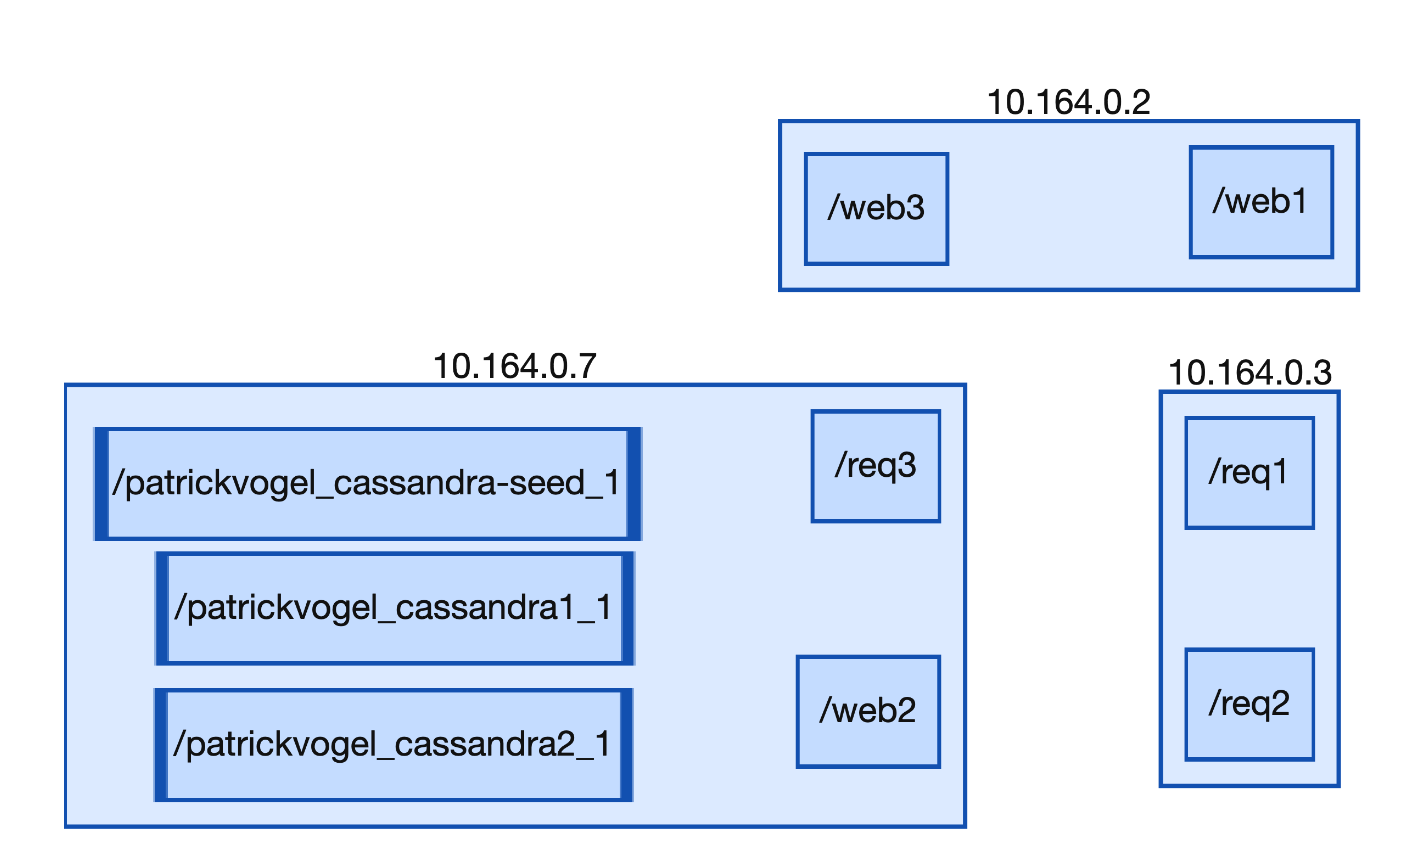
\includegraphics[width=\textwidth]{gfx/demo_app}
    \caption{All containers in the demo application}
    \label{fig:demo_app}
\end{figure}

\noindent
In this demo application it is easy to interpret the cost model of the system. The supernode consumes almost all its CPU resources, but barely uses memory. Node $1$ is low on memory and CPU, and can therefore be used to see how the waste is distributed. Node $2$ consumes a lot of memory, but barely uses CPU. For a time period of one hour, the CPU usage is presented in \autoref{fig:demo_cpu_cost}. From this figure, we conclude hat the monitored data from our solution are in compliance with this expected behaviour. Note that the unit of the CPU usage is `CH', which means `core hour'. This represents $n_\text{CPU}$ from \autoref{eq:p}.\\

\begin{figure}
    \centering
    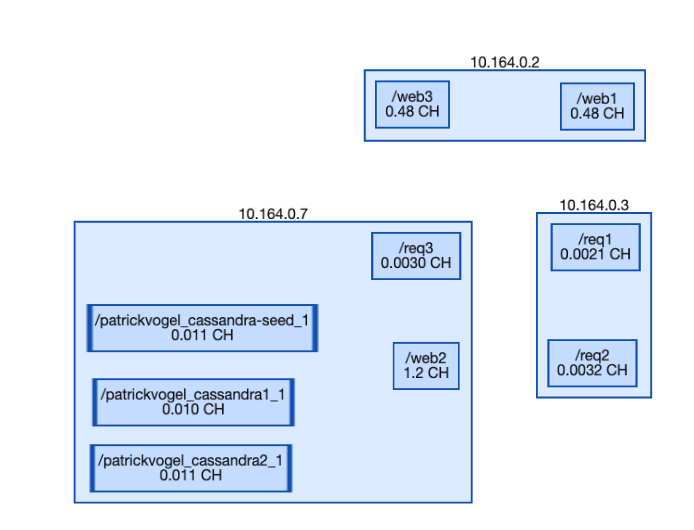
\includegraphics[width=\textwidth]{gfx/demo_cpu_cost}
    \caption{Distribution of the CPU usage for 1 hour}
    \label{fig:demo_cpu_cost}
\end{figure}

\noindent
From the CPU usage, the CPU waste is determined. This can be found in \autoref{fig:demo_cpu_waste}. Interesting is node $2$ ($10$.$164$.$0$.$7$), which shows that all containers, except for the web-service, are responsible for a lot of CPU waste. The supernode is barely responsible for waste, as the CPU usage is near $100\%$. Node $1$ has two equivalent containers, and therefore the waste is equally divided over the nodes.\\

\begin{figure}
    \centering
    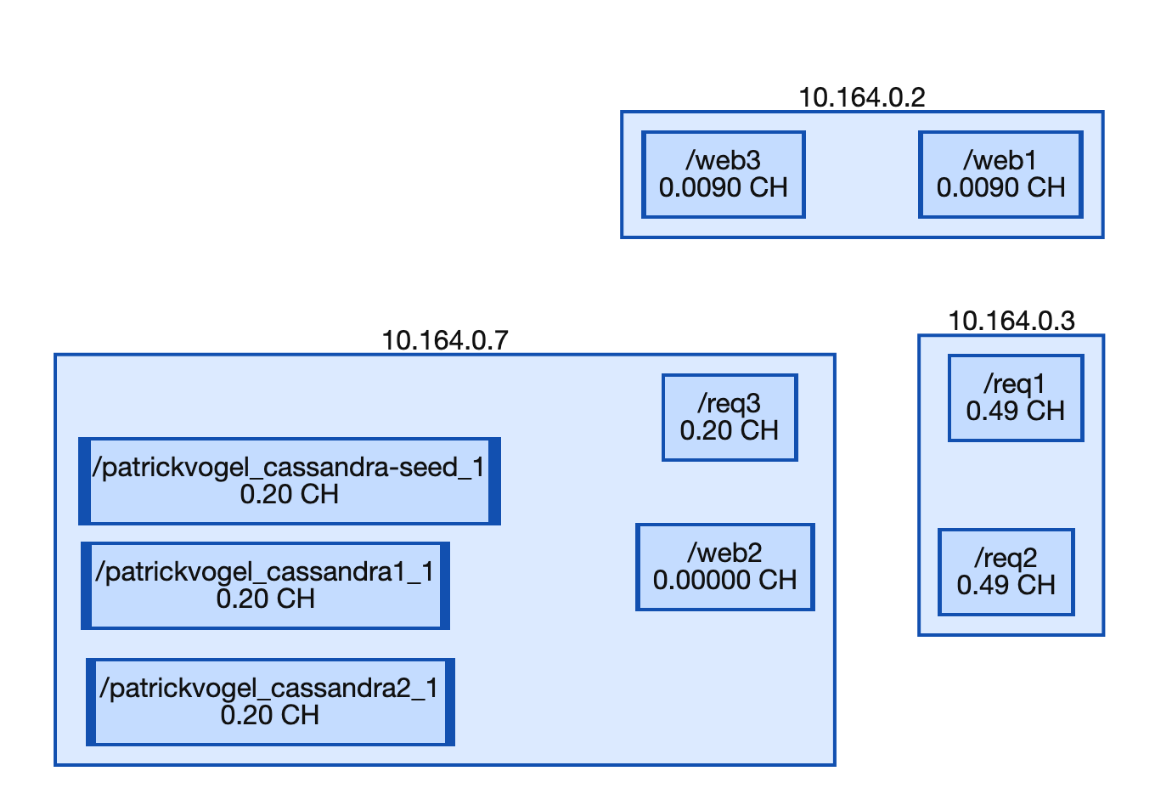
\includegraphics[width=\textwidth]{gfx/demo_cpu_waste}
    \caption{Distribution of the unused CPU for 1 hour}
    \label{fig:demo_cpu_waste}
\end{figure}

\noindent
The same analysis can be made for the memory usage- and waste-distribution. The memory usage is presented in \autoref{fig:demo_mem_cost}, and the memory waste is presented in \autoref{fig:demo_mem_waste}. As the web-services on the supernode are efficient in terms of memory usage, their corresponding waste is large. This also applies to the request-services on node $1$. The memory waste distribution is interesting on node $2$, as the three Cassandra services uses too much memory resources, and therefore don't receive any memory waste.\\

\begin{figure}
    \centering
    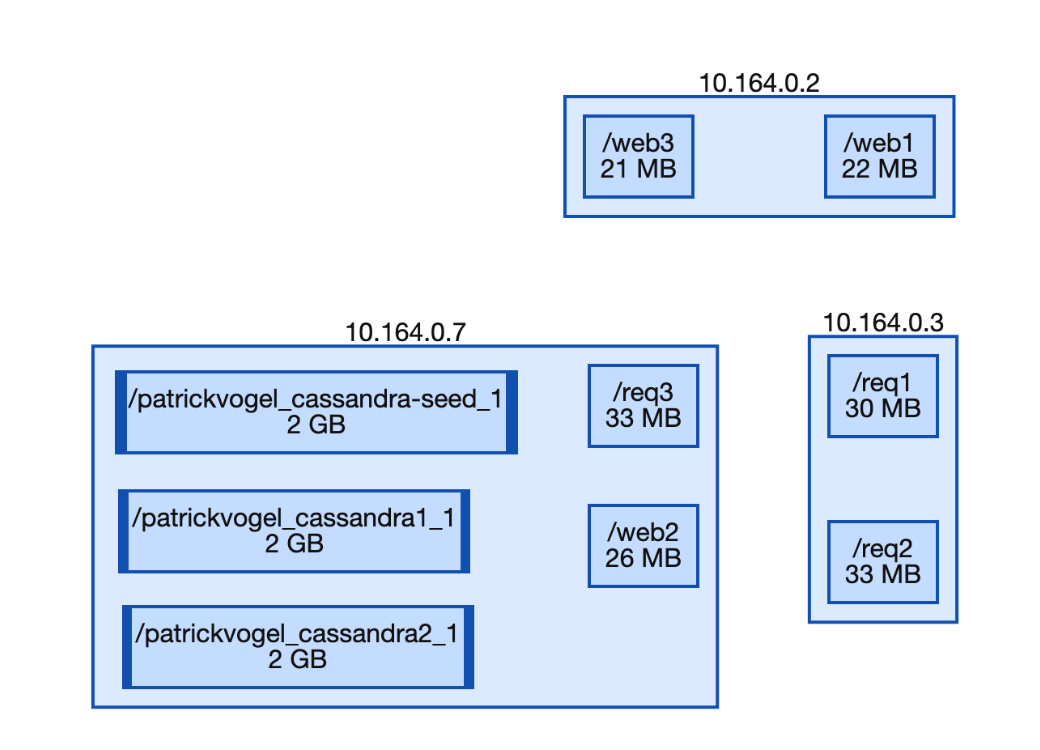
\includegraphics[width=\textwidth]{gfx/demo_mem_cost}
    \caption{Distribution of the memory usage for 1 hour}
    \label{fig:demo_mem_cost}
\end{figure}

\begin{figure}
    \centering
    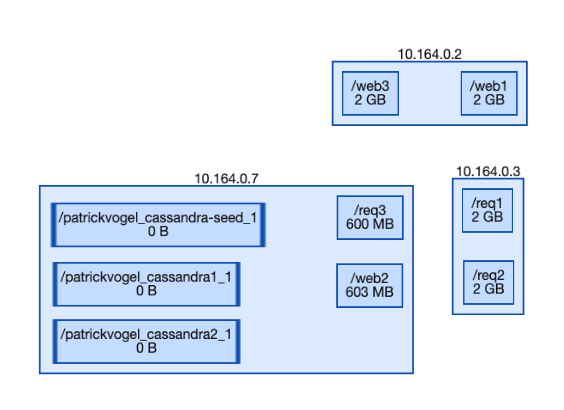
\includegraphics[width=\textwidth]{gfx/demo_mem_waste}
    \caption{Distribution of the unused memory for 1 hour}
    \label{fig:demo_mem_waste}
\end{figure}

\noindent
The network traffic analysis is shown in \autoref{fig:demo_network}. However, as all communication is internally, the amount of outgoing network is nearly zero. Due to the inaccuracy of the network analysis, it is not exactly zero, which is in \autoref{sec:eval_k}.\\

\begin{figure}
    \centering
    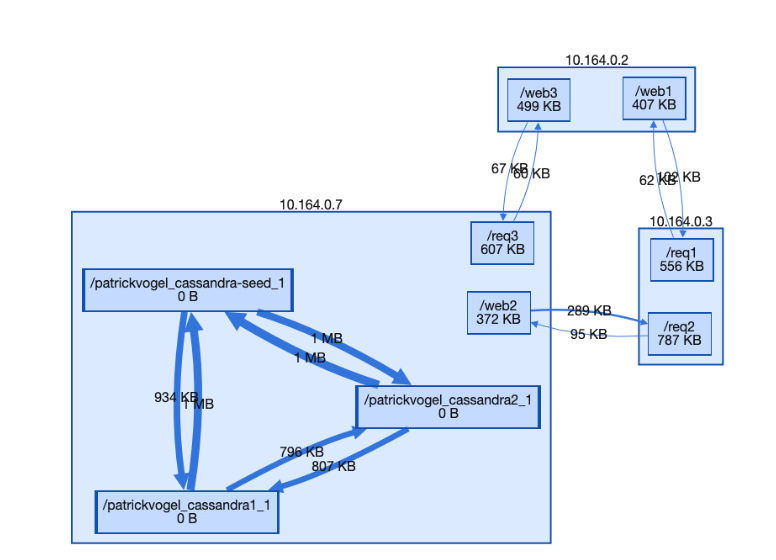
\includegraphics[width=\textwidth]{gfx/demo_network}
    \caption{Amount of outgoing network traffic for 1 hour}
    \label{fig:demo_network}
\end{figure}

\noindent
The used resources as presented in \autoref{fig:demo_cpu_cost}, \autoref{fig:demo_mem_cost} and \autoref{fig:demo_network} are used for the cost computation, which is presented in \autoref{fig:demo_cost}. This cost model is based on the following prices:
\begin{itemize}
    \item $p_\text{CPU}$: USD 0.021925 per hour per CPU per host.
    \item $p_\text{memory}$: USD 0.002938 per hour per GB memory per host.
    \item $p_\text{network}$: USD 0.10 per GB of network traffic going out of their system.
\end{itemize}

\noindent
The unused resources as presented in \autoref{fig:demo_cpu_waste} and \autoref{fig:demo_mem_waste} are used for the waste computation, which is presented in \autoref{fig:demo_waste}. The cost and waste are computed using \autoref{eq:cost_and_waste}.\\

\begin{figure}
    \centering
    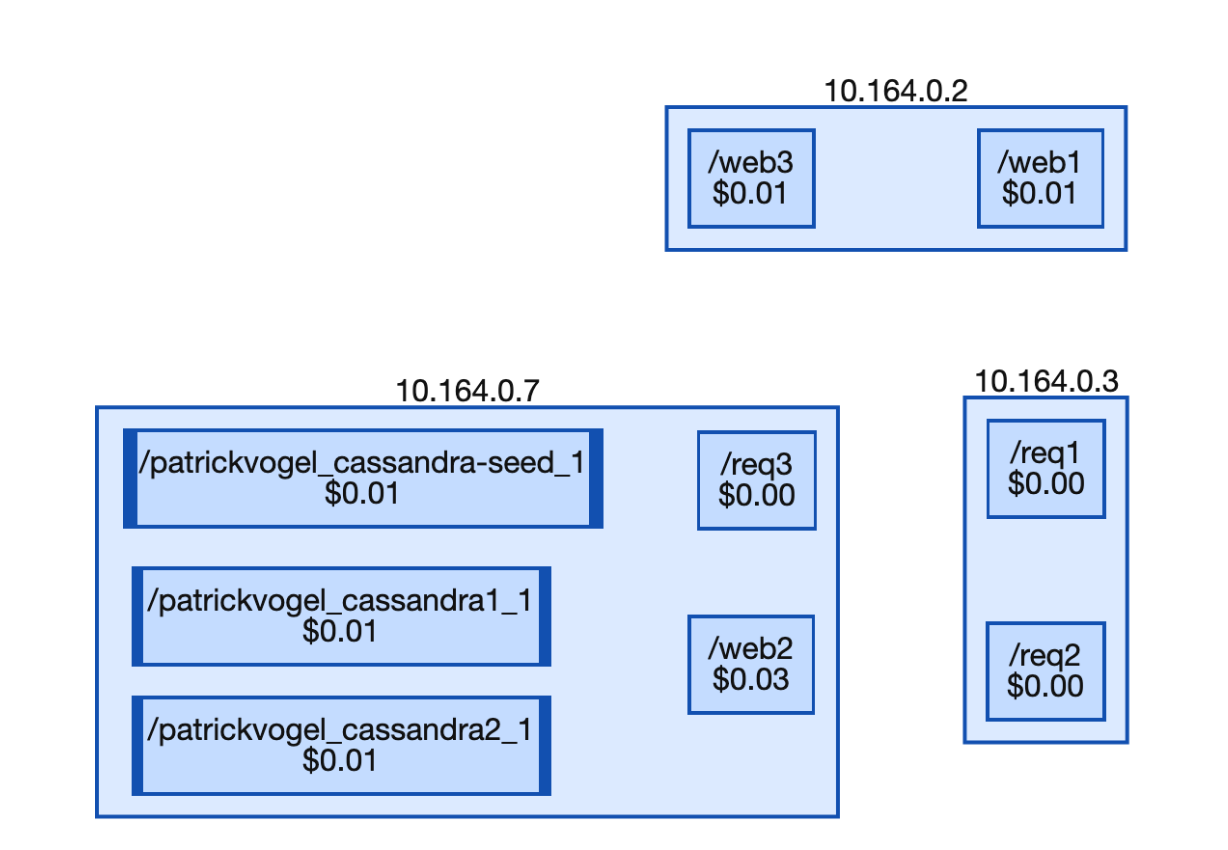
\includegraphics[width=\textwidth]{gfx/demo_cost}
    \caption{Cost per container for a period of 1 hour}
    \label{fig:demo_cost}
\end{figure}

\begin{figure}
    \centering
    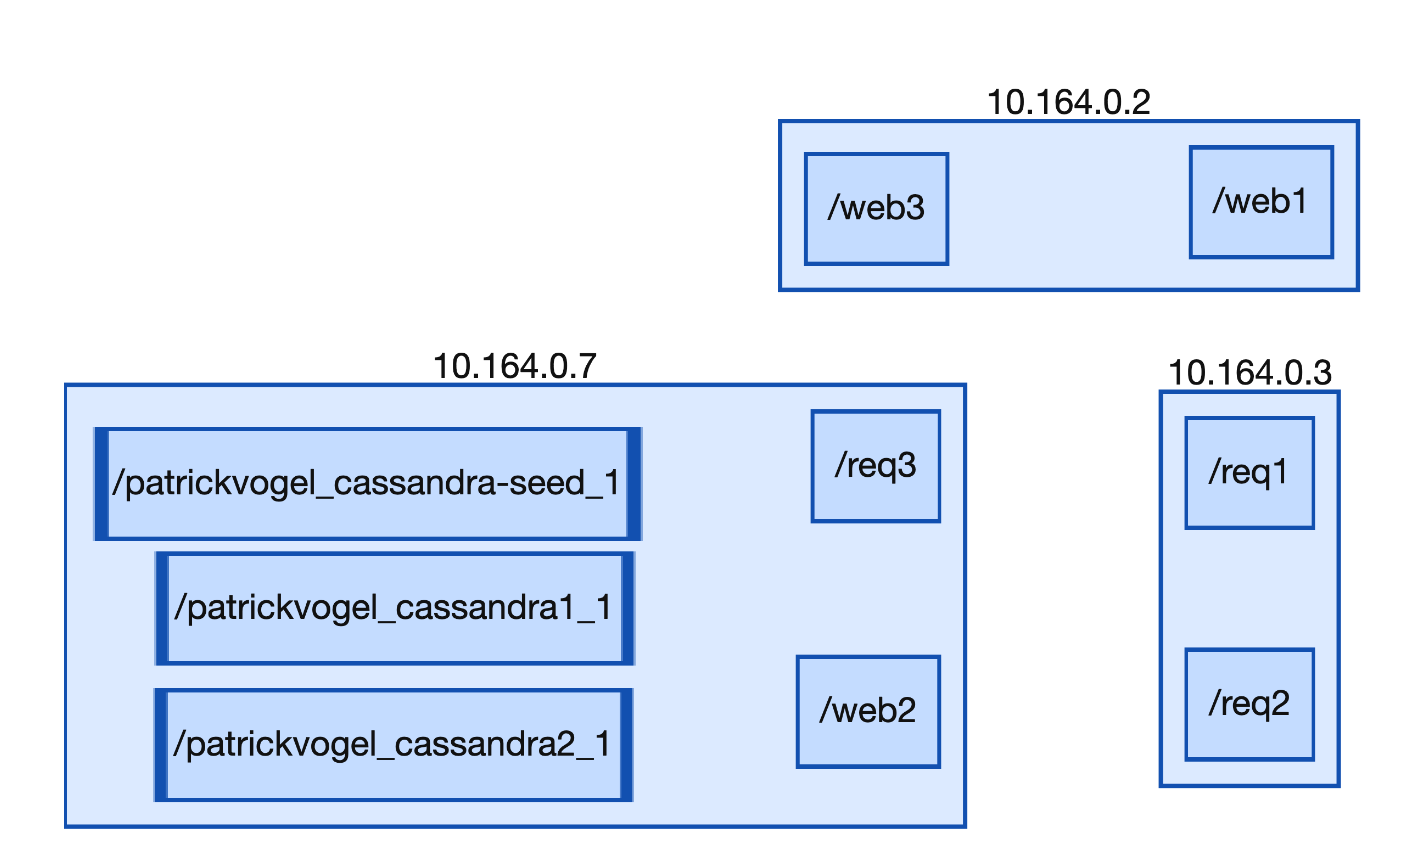
\includegraphics[width=\textwidth]{gfx/demo_app}
    \caption{Waste cost per container for a period of 1 hour}
    \label{fig:demo_waste}
\end{figure}

\noindent
In order to simplify the results, the visualizations can also be based on the groups, as determined above. This is also presented in the industrial case study and is therefore not further described in this chapter. So far, the figures above show the resource usage and cost for a specific amount of time. This already provides interesting results, but aggregating provides further simplification. The aggregated results can be found in \autoref{fig:demo_stats}.

\begin{figure}
    \centering
    \subfloat[Cost and waste values]{
        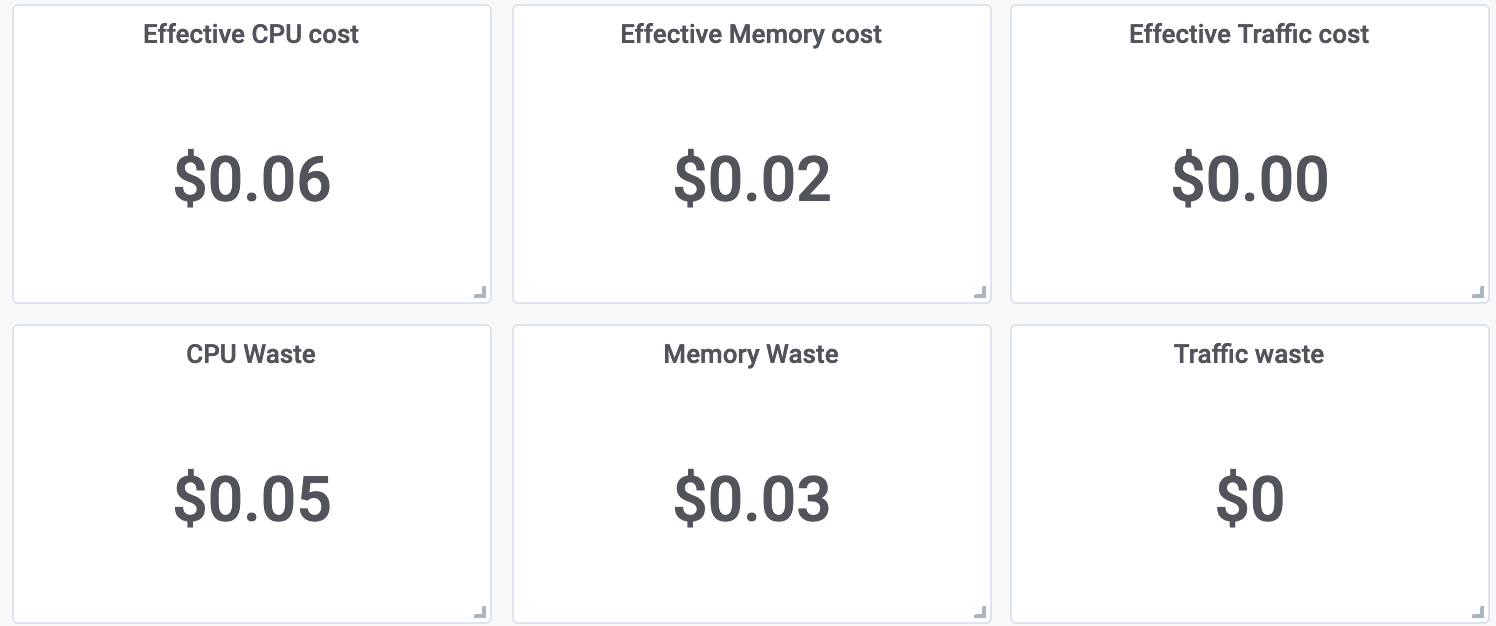
\includegraphics[width=0.45\textwidth]{gfx/demo_stats1.png}
    }
    
    \subfloat[Cost and waste ratios]{%
        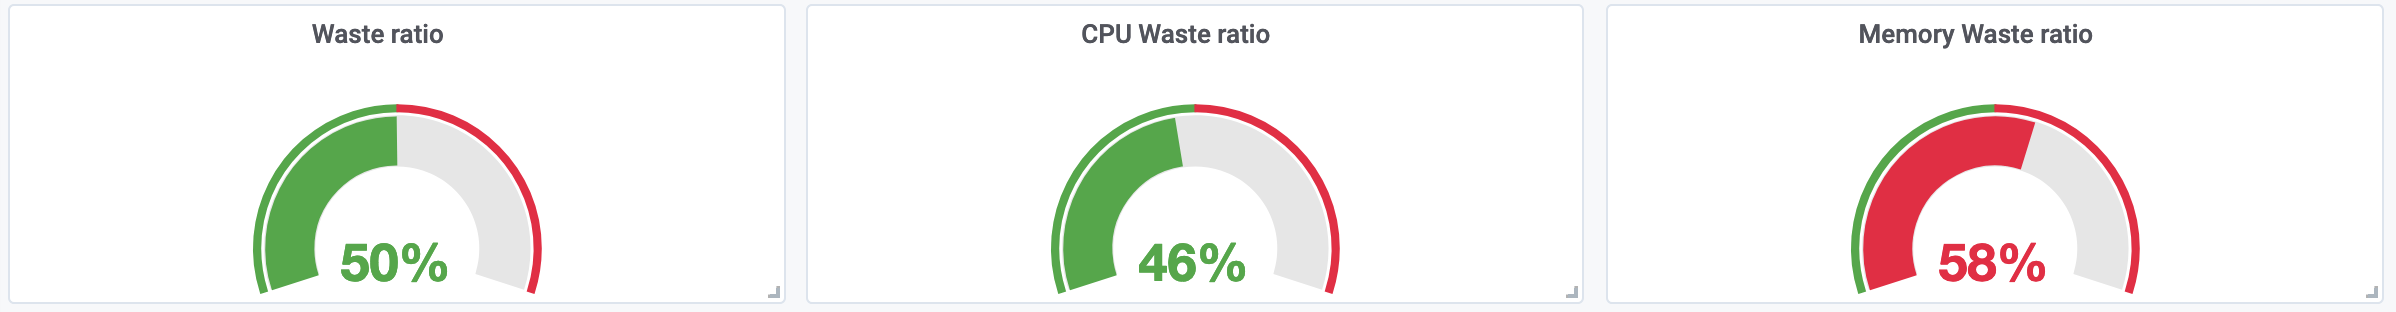
\includegraphics[width=0.45\textwidth]{gfx/demo_stats2.png}
    }
    \caption{Aggregated stats for the demo application after one hour}
    \label{fig:demo_stats}
\end{figure}